\section{Adaptive Action-Level Speculation}
\label{sec:algo}
Despite the strictly serial dependency within the search agent, we argue that action-level speculation can reduce model inference latency and overlap action-execution time to shrink the overall step latency.
In this section, we present a two-phase speculation framework that adapts to the varying reasoning demands across different steps.
By leveraging speculation differently in these two phases, the framework achieves a balanced trade-off between execution efficiency and task accuracy throughout the search task.
We will introduce the motivation, the two distinct phases, their transition mechanism, and the design of action results reuse mechanism through an Action Server.

\subsection{Motivation}
Our adaptive action-level framework is motivated by the reasoning demands vary in steps of search agents.
% Instead of waiting for model output action after thinking in the original reason-action process, we find that the model can output reasonable actions directly without reasoning.
As shown in \Figref{fig:fig1}b, we allow the model to directly sample candidate actions without reasoning.
Preliminary results indicate that these directly generated speculative actions can often match those produced after reasoning, particularly in the early steps of the task, where we observe 73.4\% match rate in the first step.
This suggests that in the initial stages, where the agent primarily extracts key entities or keywords for search, the reasoning demand is relatively low, and effective actions can be inferred without deep thought.

However, as the task progresses and the agent must integrate accumulated information to plan accurately, deliberate reasoning becomes essential for generating coherent and correct actions.
As an evidence, the speculative action hit rate falls to as low as 11\% in later steps.
Based on this, we design two specific phases to address these different characteristics:
\begin{itemize}[leftmargin=*]
    \item In the \textbf{Aggressive Speculation Phase} (low reasoning complexity), the agent employs speculation to skip reasoning and directly predict actions, thereby reducing the \textit{inference time} spent on thought generation.
    \item In the \textbf{Verified Speculation Phase} (high reasoning complexity), the agent performs reasoning while concurrently applying speculation to predict and execute likely actions in parallel, thereby overlapping the \textit{action execution time}.
\end{itemize}

\begin{figure}
    \centering
    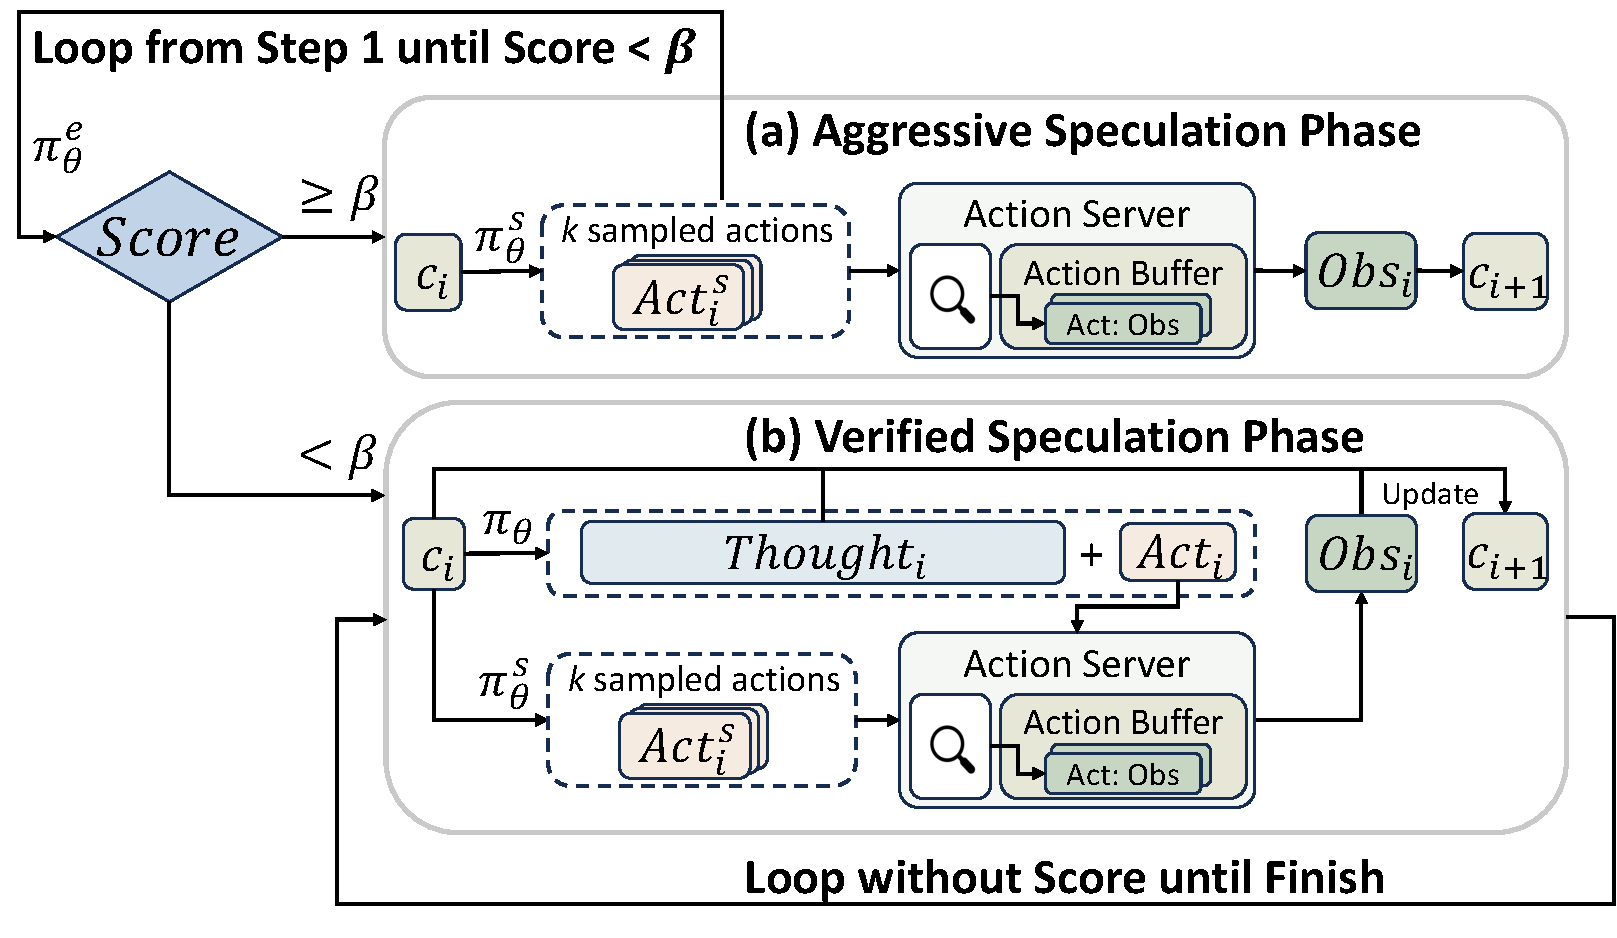
\includegraphics[width=0.95\linewidth]{figures/phase_switch.pdf}
    % \vspace{-10pt}
    \caption{Adaptive Speculation in search agents.}
    % \vspace{-12pt}
    \label{fig:ada_spec}
\end{figure}

\subsection{Aggressive Speculation Phase}
\label{sec:aggressive}
This phase appears in the early steps of the search agents, where the reasoning demand is low, direct speculation for actions can get reasonable results.
As shown in \Figref{fig:ada_spec}a, given the current context $c_i$, the agent directly samples $k$ speculative actions through model inference $\pi_{\theta}^s$.
After that, the agent gets the observation result of sampled actions through the Action Server, which contains the search API and Action Buffer to store the action results for speculation. 
We will introduce them in detail in the \Secref{sec:action-server}.
Compared to the original reason-action step in the search agent, the steps in the Aggressive Speculation Phase effectively reduce the latency of reasoning in the model inference.

\subsection{Verified Speculation Phase}
\label{sec:verified}

To complement the Aggressive Speculation Phase and preserve accuracy in reasoning-intensive steps, we introduce the Verified Speculation Phase, where speculation runs alongside normal reasoning.
At each step in \Figref{fig:ada_spec}b, the agent generates the $(Thought, Act)$ pair on the main agent path, while a parallel speculative path samples $k$ candidate actions and executes them immediately.
If a speculative action matches the action later produced in main agent path, its execution result is retrieved directly from the Action Server.
Otherwise, the main path falls back to executing the correct one.

Compared with the original step in the search agent, the steps in Verified Speculation Phase add additional speculation for actions and therefore enable the parallelization between model reasoning in main agent path and action execution in speculative path.
However, this speculation strategy adds extra requests to the model inference system, which may lead to degradation in inference speed, especially in high-concurrency scenarios.
We will tackle this problem in \Secref{sec:intra-sched}.

\begin{figure}[t]
    \centering
    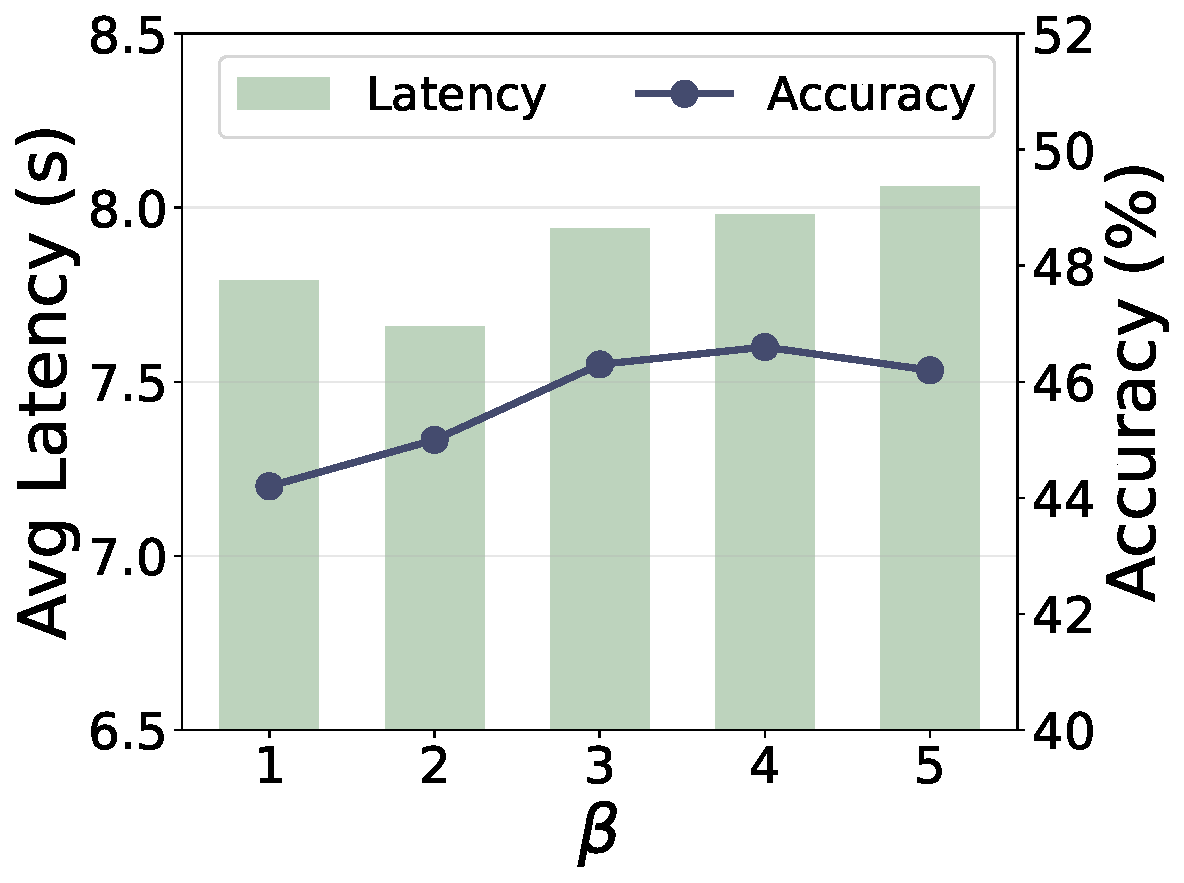
\includegraphics[width=0.5\linewidth]{figures/experiments/beta_analysis.pdf}
    \caption{Influence of $\beta$ on accuracy and latency.}
    \label{fig:beta}
\end{figure}

\subsection{Phase Transition}
While each speculation phase offers distinct benefits: 
Aggressive Speculation reduces inference time by omitting reasoning, and Verified Speculation ensures accuracy through reasoning-guided verification and overlaps action execution time. 
Using either mode alone across the entire task is inaccurate or inefficient. 
To adaptively balance efficiency and accuracy, we introduce a dynamic switching mechanism based on the agent's self-reflection~\cite{reflexion}. 
As shown in \Figref{fig:ada_spec} left, after generating speculative actions in the Aggressive Speculation Phase, we invoke an inference call ($\pi_\theta^e$) to score their plausibility.
When all scores of $k$ speculative actions fall below a predefined threshold $\beta$, the system interprets this as a signal that the task has entered a reasoning-intensive stage and transitions to the Verified Speculation Phase. 
This adaptive design allows the agent to skip unnecessary reasoning in the early steps while leveraging verified parallel speculation in later steps, effectively reducing latency without compromising accuracy.

We show the influence of threshold choice in this switching mechanism using Gemma-3-27B on the 2WikiMultiHopQA benchmark, as shown in \Figref{fig:beta}.
Using a 1-5 scoring scale, we observe a clear trade-off: increasing $\beta$ improves answer accuracy but also increases average latency. 
Notably, accuracy gains saturate once $\beta\!>\!3$, while latency continues to grow. 
The results suggest that $\beta\!=\!3$ or $4$ provides the best balance, enabling early-step fast speculation while reliably switching to verified reasoning in complex stages.

\subsection{Action Server}
\label{sec:action-server}
The Action Server is the system component that enables reuse of speculative execution results.
It maintains an in-memory Action Buffer that is implemented as a thread-safe dictionary mapping actions to their execution states and results.
The buffer resides entirely in CPU memory, and its footprint remains small in practice, about 200 Bytes per task.
Incoming action requests are handled concurrently: upon arrival, the server checks the buffer to determine whether the action is already completed or in progress.
If so, the request reuses the stored result or attaches to the ongoing execution, avoiding redundant tool latency.
Only actions absent from the buffer trigger a new search API call.
This design allows the main agent path to immediately consume pre-executed speculative results while ensuring correct synchronization under parallel execution.

